\documentclass[11pt, oneside]{article}   	% use "amsart" instead of "article" for AMSLaTeX format
\usepackage{geometry}                		% See geometry.pdf to learn the layout options. There are lots.
\geometry{letterpaper}                   		% ... or a4paper or a5paper or ... 
\usepackage{graphicx}				% Use pdf, png, jpg, or eps§ with pdflatex; use eps in DVI mode
								% TeX will automatically convert eps --> pdf in pdflatex		
\usepackage{amssymb}
\usepackage{amsmath}
\usepackage{parskip}
\usepackage{color}
\usepackage{hyperref}

\graphicspath{{/Users/telliott_admin/Dropbox/Tex/png/}}
% \begin{center} 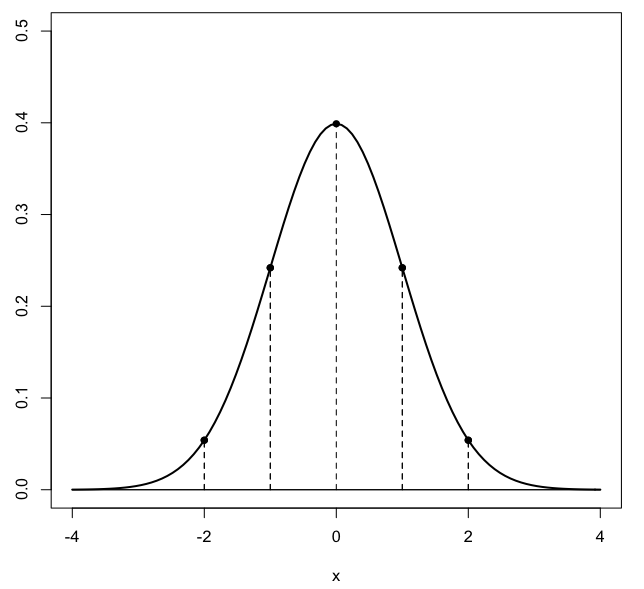
\includegraphics [scale=0.4] {gauss3.png} \end{center}

%break
\title{Newton}
\date{}

\begin{document}
\maketitle
\Large

\label{sec:Newton}

\begin{center} 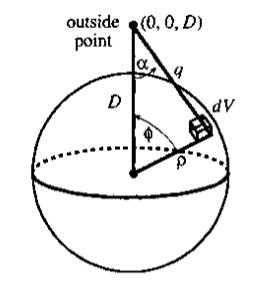
\includegraphics [scale=0.75] {Strang_14_18.png} \end{center}

Strang introduces a problem solved by Newton which, it has been argued, delayed the publication of his results since he could not justify a central assumption of gravitational theory.

The result is that the mass of a sphere acts (gravitationally) as if it is a point mass at the center of the sphere.  

We will solve this problem in two ways.  First, by working through it as set up by Strang and using his hints. 

Our second approach will use the "shell theorem" as given in wikipedia, an approach that at first seems quite different than Strang's.  However, in both approaches, as we will see, the law of cosines is center stage, and the equations simplify dramatically in a way that is oddly parallel.

Strang's figure is shown above.  In the figure, we consider the gravitational force at the point $(0,0,D)$, which is at a distance $D$ from the center of the sphere. The center of the sphere is placed at the origin.  

$\phi$ is the usual polar angle to a little element of volume $dV$, which is a distance $q$ from our point.  $\alpha$ is the angle between the radial vector and the vector from us to the element $dV$ (it is \emph{not} $90^\circ - \phi$).
\begin{center} 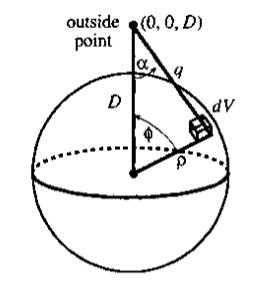
\includegraphics [scale=0.5] {Strang_14_18.png} \end{center}

As Strang explains, what we need is the average of $1/q$ over the whole volume (not the average $\bar{q}$), and this turns out to  be $1/D$.  Thus, the gravitational potential $f$ is \
\[ f = \iiint\limits_{\text{sphere}} \frac{1}{q} \ dV = \frac{V}{D} \]

Then Strang says that the gravitational force is the gradient of $f$, written $\nabla f$, and its $z$-component is
\[ f_z = -\frac{V}{D^2} = \iiint\limits_{\text{sphere}}  \ \frac{1}{q^2} \ \cos \alpha \ dV \]

In other words, the average value of $1/q^2$ multiplied by $\cos \alpha$, works out to be equal to $1/D^2$, which seems remarkable.

What we want to do here is follow his work on the first integral and then see if we can figure out the second one, which he "leaves for us."

\subsection*{integral for the potential}
We will do this integral in the order $d\theta \ d\phi \ d\rho$, starting with $\theta$.  That is:
\[ \int_{\rho = 0}^{R} \int_{\phi = 0}^{\pi} \int_{\theta=0}^{2\pi} \frac{1}{q} \ \rho^2 \sin \phi \ d\theta \ d\phi \ d \rho \]

I'm assuming this is basically familiar.

The inside integral gives a factor of $2 \pi$, which we'll forget about for the moment and put back in at the end.  And we'll do the outside integral just before that.  

So we have to solve
\[ \int_{\phi = 0}^{\pi} \frac{1}{q} \ \rho^2 \sin \phi \ d\phi  \]

We need an expression for $q$.  
\begin{center} 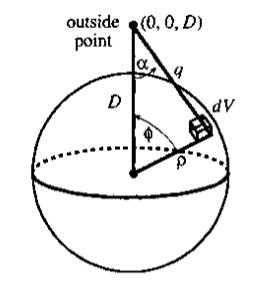
\includegraphics [scale=0.5] {Strang_14_18.png} \end{center}
By the law of cosines
\[ q^2 = D^2 + \rho^2 - 2 D \rho \cos \phi \]

This is probably a good place for a substitution!  Let
\[ u = q^2 \]
\[ = D^2 + \rho^2 - 2 D \rho \cos \phi  \]
and then
\[ du = 2 D \rho \ \sin \phi \ d \phi \]
\[ \frac{1}{2D} \ du =  \rho \sin \phi \ d \phi \]
\subsection*{substitution}

we have
\[ \int_{\phi = 0}^{\pi} \frac{1}{q} \ \rho^2 \sin \phi \ d\phi  \]
\[ = \frac{1}{2D}  \ \rho \int \frac{1}{\sqrt{u}} \ du\]
\[ =  \frac{\rho}{D}  \ \sqrt{u} \]
\[ =  \frac{\rho}{D}  \ \sqrt{D^2 + \rho^2 - 2 D \rho \cos \phi} \]

Leave aside the factor of $\rho/D$ for the moment.  We need to evaluate the $\sqrt{u}$ plugging in the value for $\cos \phi$ at the bounds.

These are
\[ \phi = 0 \rightarrow \pi \]
so
\[ \cos \phi \ \bigg |_0^{\pi} \]
This gives $1$ at the lower bound and $-1$ at the upper one.

Thus, with subtraction (evaluating at the upper bound and then subtracting the result for the lower bound)
\[ \sqrt{D^2 + \rho^2 + 2 D \rho} - \sqrt{D^2 + \rho^2 - 2 D \rho}  \]
we obtain two perfect squares
\[ \sqrt{(D + \rho)^2} - \sqrt{(D - \rho)^2}  \]
\[ (D + \rho) - (D - \rho) = 2 \rho \]

So, recalling the extra factor of $\rho/D$, the middle integral becomes simply
\[ = \frac{2 \rho^2}{D} \]
Remember the factor of $2 \pi$
\[ = \frac{4 \pi \rho^2}{D} \]

Then, the outer integral is
\[ \int_0^R \frac{4 \pi \rho^2}{D}  \ d\rho = \frac{4}{3} \frac{ \pi R^3}{D} = \frac{V}{D} \]
as we said.  The average value of the expression $1/q$ over the whole volume is equal to $1/D$.

\subsection*{integral for the force}
The second half of the problem is the force.  We want the component of it directed along the $z$-axis, so multiplying by factor of $\cos \alpha$.
\begin{center} 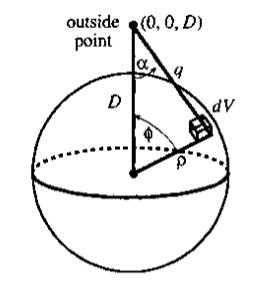
\includegraphics [scale=0.5] {Strang_14_18.png} \end{center}

Strang says to calculate
\[  \iiint\limits_{\text{sphere}} \frac{1}{q^2} \ \cos \alpha \ dV \]
and we should obtain
\[ \frac{\text{V}}{D^2} \]
The average value of $1/q^2$ together with that factor of $\cos \alpha$ somehow works out to be $1/D^2$.

The hint is to use the law of cosines again, both to deal with $\cos \alpha$ as well as $\sin \phi$.

We start with
\[ \rho^2 = D^2 + q^2 -2Dq \cos \alpha \]
so 
\[ \cos \alpha = \frac{1}{2Dq} (D^2 + q^2 -\rho^2) \]

and the integral is then
\[  \iiint\limits_{\text{sphere}} \frac{1}{q^2} \ \cos \alpha \  dV \]
\[  \frac{1}{2D}  \iiint\limits_{\text{sphere}} \frac{1}{q^2} \cdot \ \frac{D^2 + q^2 -\rho^2}{q}  \ dV \]
\[  = \frac{1}{2D}  \int_{\rho = 0}^{R} \int_{\phi = 0}^{\pi} \int_{\theta=0}^{2\pi} \frac{D^2 + q^2 -\rho^2}{q^3}  \ \rho^2 \ \sin \phi  \ d \phi \]

The inner integral with respect to $\theta$ will give $2 \pi$ as before (which we leave aside for now), and waiting to do the outer integral with respect to $\rho$, the middle integral is
\[ \frac{1}{2D} \int_{\phi = 0}^{\pi}  \frac{D^2 + q^2 -\rho^2}{q^3} \ \rho^2 \ \sin \phi \ d \phi \]

We need to deal with those $q$'s.  Let 
\[ u = q^2 = D^2 + \rho^2 - 2 D \rho \cos \phi \]
\[ du = 2 D \rho \ \sin \phi \ d \phi \]
treating $\rho$ is fixed for this middle integral.
\[ \frac{1}{2D} \ du = \rho \sin \phi \ d \phi \]
We had
\[ \frac{1}{2D} \int_{\phi = 0}^{\pi}  \frac{D^2 + q^2 -\rho^2}{q^3} \ \rho^2 \ \sin \phi \ d \phi \]
which becomes
\[ \frac{1}{2D}  \int  \frac{D^2 + u -\rho^2}{u^{3/2}} \ \rho \ \frac{1}{2D} \ du \]
\[ = \frac{\rho}{4D^2}  \int  \frac{D^2 + u -\rho^2}{u^{3/2}} \  \ du \]
\[ = \frac{\rho}{4D^2} \ [ \ \int  \frac{D^2 -\rho^2}{u^{3/2}} \  \ du + \int  \frac{1}{\sqrt{u}} \ du \ ] \  \]
The integral isn't bad:
\[ = \frac{\rho}{4D^2} \ [ \ (D^2 - \rho^2) \frac{(-2)}{\sqrt{u}} + 2 \sqrt{u}   \ ] \]
Rather than reverse the substitution, recall the bounds
\[ \cos \phi \ \bigg |_0^{\pi} \]
which give $1$ at the lower bound and $-1$ at the upper one.

Recall 
\[ u = q^2 = D^2 + \rho^2 - 2 D \rho \cos \phi \]
Evaluating $\sqrt{u}$ at the upper bound we have
\[ \sqrt{D^2 + \rho^2 + 2 D \rho} \]
\[ = \sqrt{(D + \rho)^2} \]
\[ = D + \rho \]
and at the lower bound we have
\[ \sqrt{D^2 + \rho^2 - 2 D \rho} = D - \rho \]

Thus, for the whole expression at the upper bound we have
\[ \frac{\rho}{4D^2} \ [ \ (D^2 - \rho^2) \frac{(-2)}{D + \rho} + 2 (D + \rho) \ ] \]
\[ =  \frac{\rho}{4D^2} \ [ \ (-2)(D - \rho) + 2 (D + \rho) \ ] \]
\[ = \frac{\rho^2}{D^2} \]

And at the lower bound
\[ \frac{\rho}{4D^2} \ [ \ (D^2 - \rho^2) \frac{(-2)}{D - \rho} + 2 (D - \rho) \ ] \]
\[ = \frac{\rho}{4D^2} \ [ \ (-2)(D + \rho) + 2(D - \rho) \ ] \]
\[ = - \frac{\rho^2}{D^2} \]

Subtracting this from the value at the upper bound yields
\[ \frac{2 \rho^2}{D^2} \]

The outer integral is then just
\[ \int_0^R  \frac{2 \rho^2}{D^2}   d \rho \]
\[ = \frac{1}{D^2} \ 2 \int_0^R  \rho^2  d \rho \]
\[ = \frac{1}{D^2} \ \frac{2}{3} R^3 \]
multiply by the last factor of $2 \pi$ and we obtain
\[ = \frac{1}{D^2} \ \frac{4}{3} \pi R^3 \]
which is just the volume divided by $D^2$, as required.\

\section*{Shell Theorem}

Wikipedia has a beautiful derivation of the "shell theorem," which says that the mass of a spherical object acts in gravitation as if the entire mass $M$ were concentrated at the center.

\url{http://en.wikipedia.org/wiki/Shell_theorem}

In this write-up, we will show that this is true for a shell of radius $R$.  Having done that, if we visualize the solid ball as a series of concentric shells, we will have the full theorem.
\begin{center} 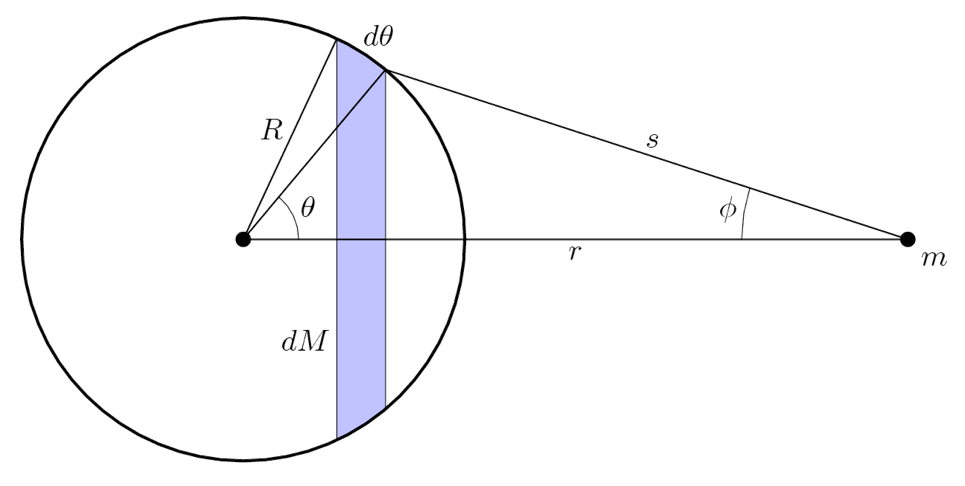
\includegraphics [scale=0.35] {shell_thm.png} \end{center}
The figure shows a cross-section of the shell.

We start by calculating the force due to a ring of mass contained inside the angular width $d \theta$, measured from the center of the shell

Using $\theta$ as the variable here is a great idea, because the mass is proportional to the area of the shell along this ring, and the width of the slice is $R \ d \theta$.

The radius of the ring is $R \sin \theta$, so the total surface area is
\[ dA = 2 \pi R \sin \theta R \ d \theta \]

The mass per unit area is the total mass $M$, divided by the surface area of the sphere
\[ \frac{M}{4 \pi R^2} \]
so the mass of the ring is the mass per unit area times the area for the ring
\[ M_r = \frac{M}{4 \pi R^2} \ 2 \pi R \sin \theta R \ d \theta \]
\[ = \frac{M}{2} \sin \theta \ d \theta \]

Each small piece of the ring has mass $dM$ and lies at a distance $s$ from the test mass $m$.
\begin{center} 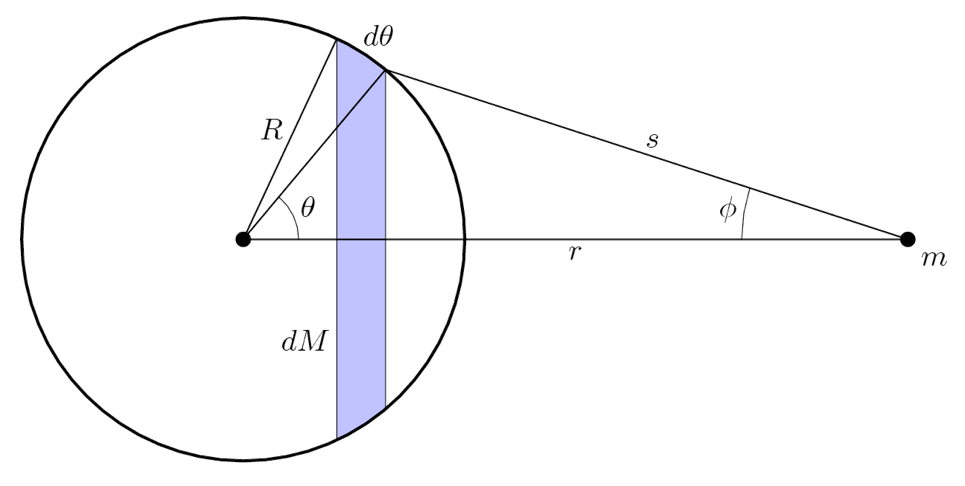
\includegraphics [scale=0.35] {shell_thm.png} \end{center}
It exerts a force of 
\[ dF = \frac{m G \ dM}{s^2} \]

The second critical insight is that for each piece the force has two components.  One acts along a line from the center of the sphere.

The other component cancels, because on the opposite side of the ring there is another small piece with the same force, but in the opposite direction.

The magnitude of the radial part is
\[ dF_r = dF \cos \phi = \frac{mG \cos \phi}{s^2} \ dM \]

(the force points toward the center of the shell, but in what follows I will work just with the magnitude.  You can pretend there is a unit radial vector coming along in all the calculations).

The total radial force is obtained by substituting the mass of the ring
\[ dF_r = \frac{mG \cos \phi}{s^2} \ \frac{M}{2} \sin \theta \ d \theta \]
\[ = \frac{GmM}{2} \frac{1}{s^2} \ \cos \phi \sin \theta \ d \theta \]

We should integrate from $\theta = 0 \rightarrow \pi$ to get the whole thing.

\subsection*{law of cosines}
While the above equation sounds nice, the trouble is that it contains three variables:  $s, \phi$, and $\theta$.  

However, the law of cosines will come to the rescue.  We write two formulas:

\[ R^2 = s^2 + r^2 - 2rs \cos \phi \]
\[ \cos \phi = \frac{s^2 + r^2 - R^2}{2rs} \]
and
\[ s^2 = R^2 + r^2 - 2rR \cos \theta \]
\[ \cos \theta = \frac{R^2 + r^2 - s^2}{2rR} \]

We need $\sin \theta$.  Differentiate the second equation (implicitly)
\[ -\sin \theta \ d \theta = -\frac{2s}{2rR} \ ds  \]
\[ \sin \theta \ d \theta = \frac{s}{rR} \ ds \]

The equation that we had was
\[ dF_r = \frac{GmM}{2} \frac{1}{s^2} \ \cos \phi \sin \theta \ d \theta \]

substitute for $\sin \theta \ d \theta$
\[ dF_r = \frac{GmM}{2} \frac{1}{s^2} \ \cos \phi \ \frac{s}{rR} \ ds \]
substitute for $\cos \phi$
\[ dF_r = \frac{GmM}{2} \ \frac{1}{s^2} \ \frac{(s^2 + r^2 - R^2)}{2rs} \ \frac{s}{rR} \ ds \]
\[ =  \frac{GmM}{4R r^2} \ \frac{(s^2 + r^2 - R^2)}{s^2} \ ds \]
\[ =  \frac{GmM}{4R r^2} \ (1 + \frac{(r^2 - R^2)}{s^2}) \ ds \]

The integral is
\[ F_r = \int dF_r = \int \frac{GmM}{4R r^2} \ (1 + \frac{(r^2 - R^2)}{s^2}) \ ds \]
\[ =  \frac{GmM}{4R r^2} \ [ \ s -  \frac{(r^2 - R^2)}{s}) \ ]  \]

What about the limits on $s$?  When $\theta = 0$, $s = r - R$, and when $\theta = \pi$, $s = r + R$ so we have
\[ F_r = \frac{GmM}{4R r^2} \ [ \ s -  \frac{(r^2 - R^2)}{s}) \ ] \ \bigg |_{r - R}^{r +R} \]
Notice that we can factor $r^2 - R^2$
\[ F_r = \frac{GmM}{4R r^2} \ [ \ s -  \frac{(r+R)(r-R)}{s}) \ ] \ \bigg |_{r - R}^{r +R} \]
So, just looking at the part in the brackets, at the upper limit we have
\[ r + R - (r - R) = 2R \]
at the lower limit
\[ r - R - (r + R) = -2R \]
doing the subtraction 
\[ = 4R \]
and $4R$ just cancels!  We obtain
\[ F_r = \frac{GmM}{r^2} \]



\end{document}